% pdflatex new.tex %
\documentclass{article}

\usepackage{graphicx}

\title{C++ Parallel application for Traveling Salesman Problem resolution by genetic algorithm}
\author{Berti Stefano}
\date{\today}

\begin{document}
    \thispagestyle{plain}
    % Titles %
    \begin{center}
        \Large
        \textbf{C++ Parallel application for Traveling Salesman Problem resolution by genetic algorithm}

        \vspace{0.4cm}
        \large Parallel and distributed system: paradigms and models
        \\2019 / 2020

        \vspace{0.4cm}
        \textbf{Berti Stefano}

        \vspace{0.9cm}
        \textbf{Abstract}
    \end{center}
    % Abstract %
    The aim of this project is to implement a genetic algorithm for the resolution of the Traveling Salesman Problem and to parallelize it with two different mechanism:
    \begin{itemize}
	\item C++ standard threads and mutex
	\item Fastflow library
    \end{itemize}
    \section{Problem description}\label{sec:s1}

    \begin{figure}
        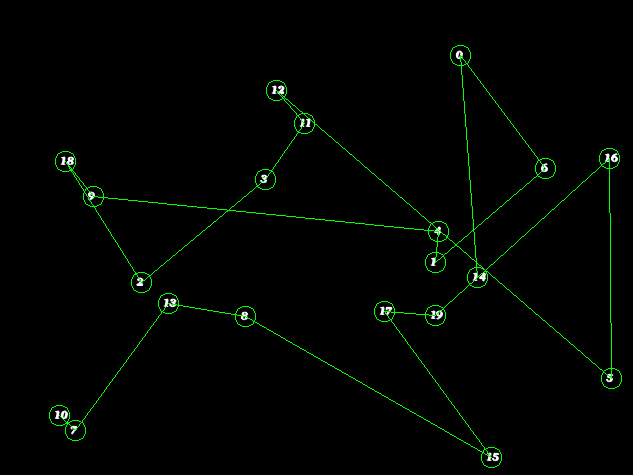
\includegraphics[width=\linewidth, height=8cm]{img/init.png}
        \caption{Initial problem with 20 nodes}
        \label{fig:init}
    \end{figure}
    \begin{figure}
        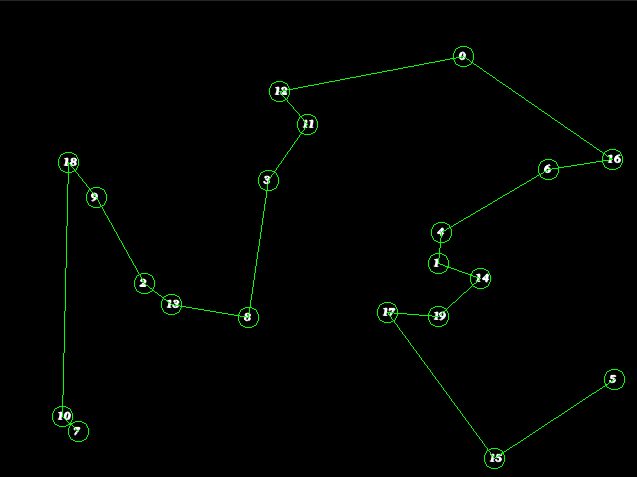
\includegraphics[width=\linewidth, height=8cm]{img/sol.png}
        \caption{Solution found after some iterations}
        \label{fig:sol}
    \end{figure}
        The genetic algorithm mimic the natural evolution and selection. In order to do that, we need a population, a way to assign a probability about which elements of the population will surivive (and so will reproduce), how they reproduce and how a mutation can occour.
	\begin{itemize}
	    \item \textbf{Population}: it is a matrix (vector of vector), where each row contains a sequence of number, and each number represent a node
	    \item \textbf{Affinity}: for each element x is the probability that x will be selected for reproduction, and is calculated as the inverse of the path length, normalized w.r.t. all other elements in order to obtain a proper probability
	    \item \textbf{Reproduction}: 2 paths A and B can create a new path C by generating 2 random numbers i and j and putting the subsequence B[i, j] in A
	    \item \textbf{Mutation}: a mutation occour with a certain probability to every generated path, and it is a random shuffle of two position in the paths. The probability that a mutation does not occour is 0.9, which is a good trade-off (too high leads to casuality, too low leads to no evolution).
	\end{itemize}
	To calculate the length of each path, I use a random generated city, where for each node number we have the relative coordinates, picked up randomly in a window of size 640x480. It is possible to plot the city and the best solution found till that moment at runtime by compiling with \textbf{make compile-graph}, this is available only for the sequential version and has huge impact on the performance, but shows the correctness of the algorithm. This algorithm is not guaranteed to find the best solution of the problem, which is a NP problem, but can find a good starting point.



    \section{A first approach}\label{sec:s2}
	The first approach that I though was a pipeline with feedback composed by a farm for calculting the length of each path, a collector to compute sum and to normalize each path length in order to obtain probability, and another farm for the reproduction stage. Each worker had its own chunk of the population/affinities to compute, and the fastflow version was implemented with a parallelforreduce to compute the sum while computing the length of each path, and a parallelfor to compute the new population. We also had some false sharing, due to the sharing of the population and affinities data structure and the modification of each worker on different part of it.
    \begin{figure}
        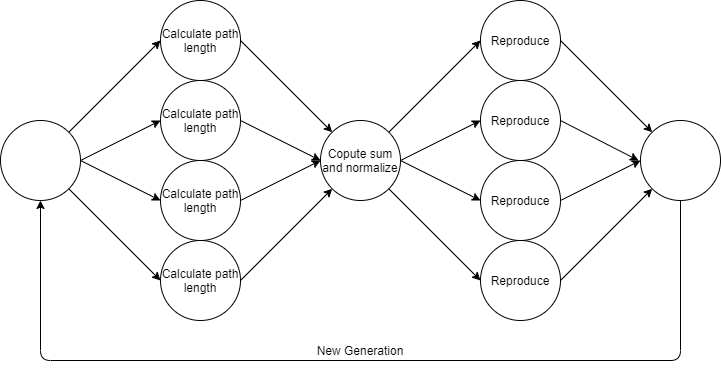
\includegraphics[width=\linewidth]{img/first.png}
        \caption{The first approach}
        \label{fig:first}
    \end{figure}
    This apporach leads to a poor speedup, because we need to stop after the calculation of the length of each member of the population in order to compute the total sum to divide them and obtain a proper probability, which will be used to select best candidates in the reproduction stage. So the good news is that we are considering a big population and the crossover between each pair of it, but the bad new is that we need to syncronize each evolution phase. But we can think to a different solution, which drives us to the normal form: when the population is big, the probabilities are all small and not very different because the path lengths don't differ too much, if we assume to have more than one independent populations, we will not make the same computation as before because we are not considering anymore the possibility of crossover among each pair og the elements of the population, but our throughtput will increase more rapidly, and we can expect a linear speedup.

    \section{The second approach}\label{sec:s3}
	This approach is a simple farm over the task \textbf{evolve}, which is a composition of the two stages \textbf{calculate affinities} and \textbf{reproduce}.
The service time of the farm is

	\centerline{$\max{T_{scheduler}, T_{w}/nw, T_{gatherer}}$}

    and the times of the scheduler and the gatherer are negligible, because the scheduler just starts the computation and the gatherer just selects the best result over the nw ones returned by the workers. So, by increasing the number of workers, I expect to see a linear speedup. My machine has 5 cores, so I also expect to have the \textbf{knee} at 5 workers. The heaviest data structure is the \textbf{population} one, which has dimension 0.8MB (4 byte(int) * 20 * 10000), while affinities has size 0.08MB (8byte(double) * 10000) and city as a very small size around 320byte (8byte(double) * 2 * 20). My cpu has 3 caches L1, L2 and L3 of size respectively 9MB, 1.5MB and 350KB, so we also expect to have a superlinear speedup at a certain point due to the population data structure fitting in the L3 cache. 
    I need to distinguish 2 cases because of I tried 2 different way to chose the elements that will be reproduced, and they give different performances. The results obtained locally are averaged on 3 runs, the results obtained on the remote machine are averaged on 5 runs.

	\subsection{Pick}\label{sec:s31}
I create a function called pick candidate, that select one element considering the probabilities. This function cost O(n) in the worst case, where n is the populaton size, because it generate a random float and decrease it with the affinities untill it becomes negative, and then select the corresponding index. When we parallelize, we divide the population size with the number of worker, and this lead not only to less element of the population to generate for each worker, but also to a reduction of the time needed to generate each element, because of the O(n) of pick candidate. So we expect something like a double of the linear speedup, motivated not only by the hardware, but because of the way I implemented the logic code.


	\subsection{Rand}\label{sec:s32}
The path length are not so different, so the affinities are almost all equal and the pick candidate function selects almost randomly the two elements of the population that will reproduce. Considering that pick candidate cost O(n) in the worst case, leading to difficultly predictable performance, I tried to replace it with a simple randomized selection of the two elements, with a cost of O(1). In this way, we can expect a linear speedup because by increasing the number of workers, we only have less elements of the population to create, but the cost to create each one is always the same.

        \begin{table}[h!]
            \begin{center}
                \caption{Expected service time, real service time, difference between the two (overhead) and relative overhead for local randomized solution with 20 nodes, 10000 size of population and 1000 iterations (time in microseconds). My machine has 5 cores.}
                \label{tab:table1}
                \begin{tabular}{c|c|c|c|c}
                    \textbf{nw} & \textbf{T(nw)} & \textbf{(T(1)/nw)} & \textbf{diff (overhead)} & \textbf{T(nw)/diff}\\
                    \hline
                        1 & 23334944 & 2341742 & 0 & 0\%\\
                        2 & 11828148 & 11667472 & 160676 & 1.3\%\\
			3 & 7937058 & 7778314 & 158743 & 2\%\\
			4 & 6065433 & 5833736 & 231697 & 3.8\%\\
			5 & 5055524 & 4666988 & 388536 & 7.6\%\\
			6 & 4975386 & 3889157 & 1086229 & 21\%\\
			7 & 5210023 & 3333563 & 1876460 & 36\%\\
                \end{tabular}
            \end{center}
        \end{table}


    \begin{figure}
        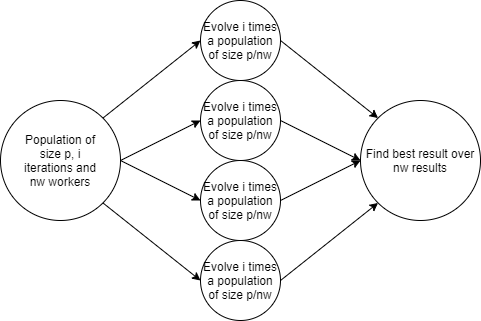
\includegraphics[width=\linewidth]{img/second.png}
        \caption{The second and final approach}
        \label{fig:second}
    \end{figure}

    \begin{figure}
        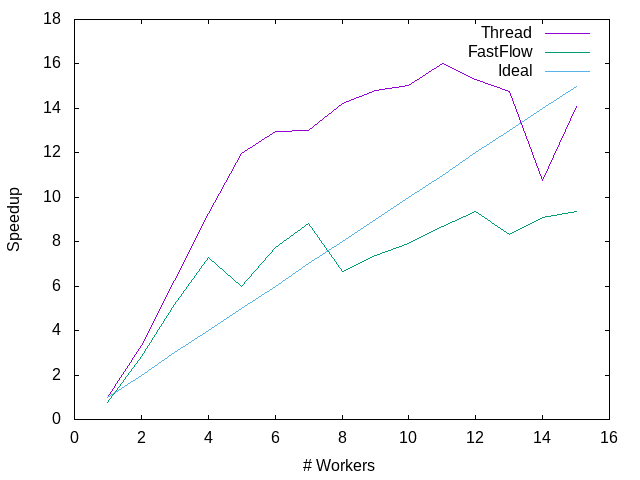
\includegraphics[width=\linewidth,height=8cm]{img/local_s_pick.png}
        \caption{Local speedup using pick candidate with 20 nodes, 10000 elements of population and 1000 iterations}
        \label{fig:local_speedup}
    \end{figure}

    \begin{figure}
        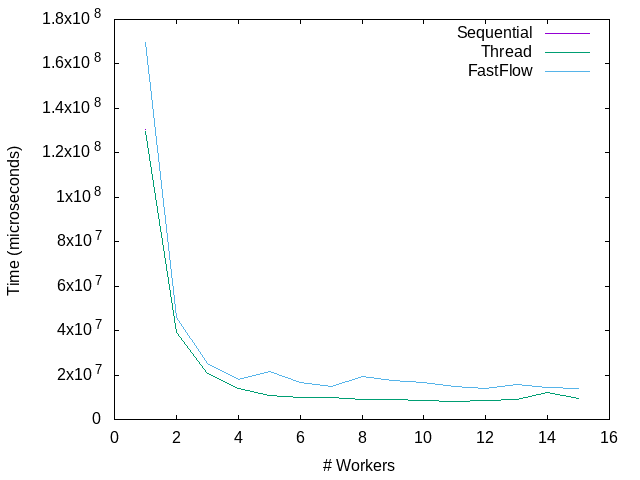
\includegraphics[width=\linewidth,height=8cm]{img/local_t_pick.png}
        \caption{Local time using pick candidate with 20 nodes, 10000 elements of population and 1000 iterations}
        \label{fig:local_time}
    \end{figure}

    \begin{figure}
        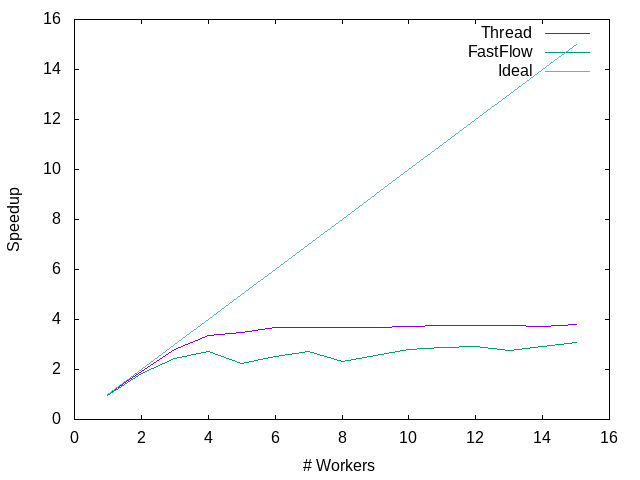
\includegraphics[width=\linewidth,height=8cm]{img/local_s_rand.png}
        \caption{Local speedup using random selection with 20 nodes, 10000 elements of population and 1000 iterations}
        \label{fig:local_speedup}
    \end{figure}

    \begin{figure}
        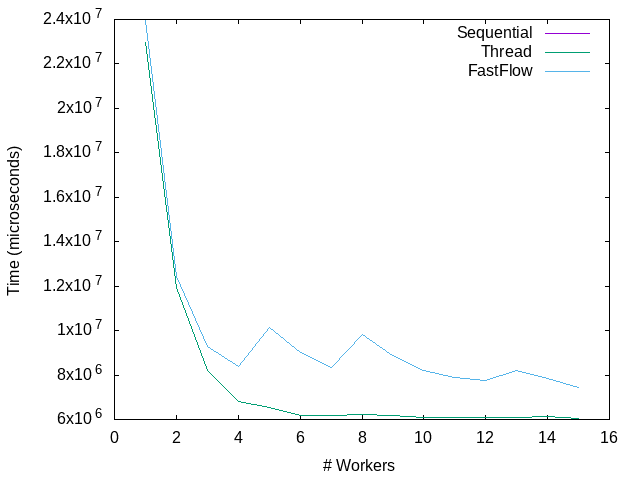
\includegraphics[width=\linewidth,height=8cm]{img/local_t_rand.png}
        \caption{Local time using random selection with 20 nodes, 10000 elements of population and 1000 iterations}
        \label{fig:local_time}
    \end{figure}

    \begin{figure}
        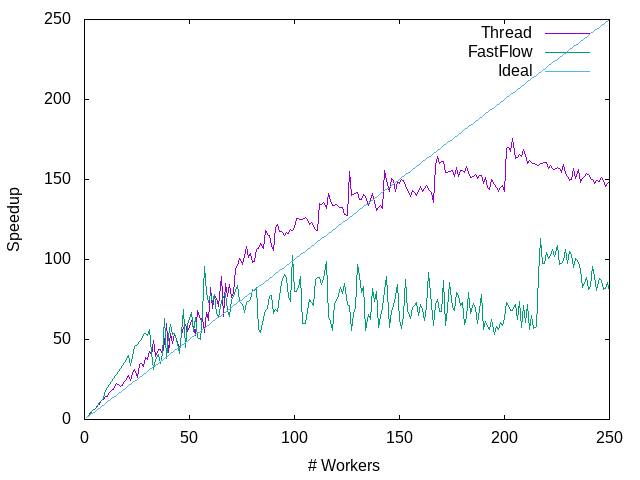
\includegraphics[width=\linewidth,height=8cm]{img/remote_s_pick.png}
        \caption{Remote speedup using pick candidate with 20 nodes, 1000 elements of population and 1000 iterations}
        \label{fig:local_speedup}
    \end{figure}

    \begin{figure}
        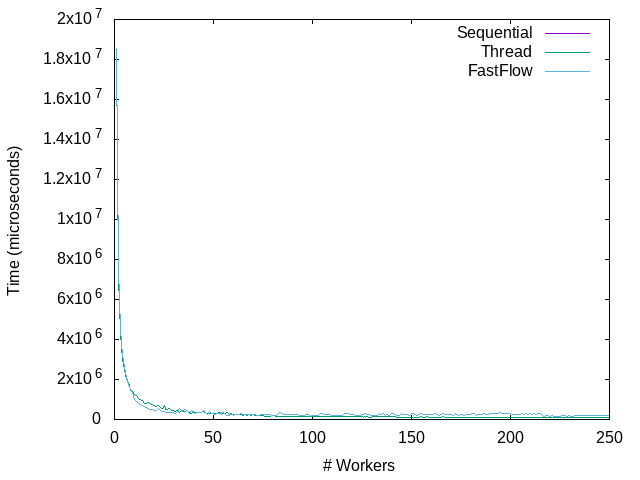
\includegraphics[width=\linewidth,height=8cm]{img/remote_t_pick.png}
        \caption{Remote time using pick candidate with 20 nodes, 1000 elements of population and 1000 iterations}
        \label{fig:local_time}
    \end{figure}

    \begin{figure}
        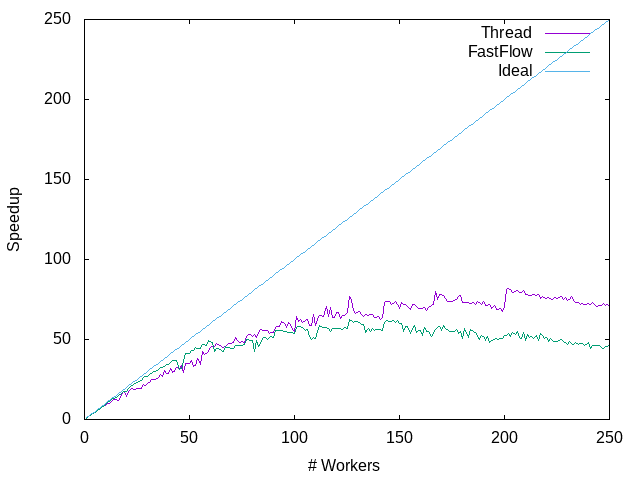
\includegraphics[width=\linewidth,height=8cm]{img/remote_s_rand.png}
        \caption{Remote speedup using random selection with 20 nodes, 1000 elements of population and 1000 iterations}
        \label{fig:local_speedup}
    \end{figure}

    \begin{figure}
        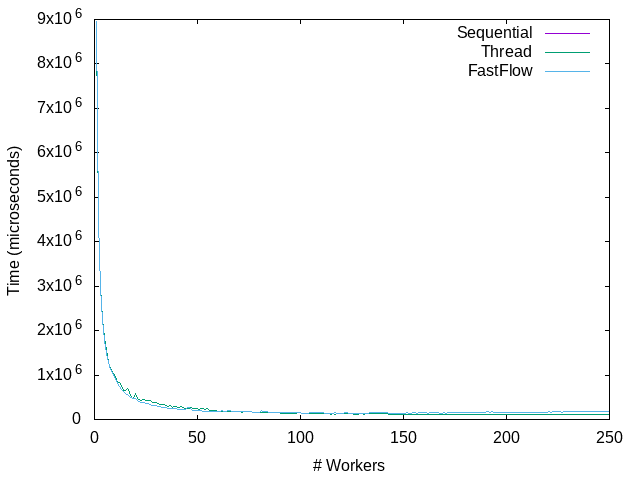
\includegraphics[width=\linewidth,height=8cm]{img/remote_t_rand.png}
        \caption{Remote time using random selection with 20 nodes, 1000 elements of population and 1000 iterations}
        \label{fig:local_time}
    \end{figure}

    \section{Difficulties}
	At a certain point, I had a bottleneck in the remote machine that doesn't allow me to have a speedup higher than 3. I investigated this problem for days to find out that my bottleneck was caused by the \textbf{rand()} function. This, together with the pick candidate, made my development and my analysis a lot more difficult. To overcome this issue, i create the MyRandom class, which sets up the 3 differents uniform distribution that I use in the program, that are [0, n\_nodes)(int), [0, pop\_size)(int) and [0, 1](double).

    \section{Other improvements}
	I always compile my code with the -O3 flag in order to make other optimizations, like vectorization, which occour in various places: when we push work in the farm of FastFlow, in the main loop of the Evolution node of FastFlow (basic block), the affinities normalization, in the main loop of the thread (basic block), in the normalization of the sequential part, in the loop that starts the thread, int the loop that generates the population. I tried to parallelize other part of the code, for example the random inizialization of the city and of the population, but I didn't get enough improvements, so I removed it.

\end{document}
